
\section{Contributions to Driftfusion}
\epigraph{\textit{"Wow, this is a gold mine!"}}

\subsection{Introduction}
During my 3-month stay in Dr.\ Piers R.\ F.\ Barnes and Prof.\ Jenny Nelson groups in Imperial College London, I utilized and expanded a modelling software developed by Dr.\ Phil Calado, Dr.\ Mohammed Azzouzi, Benjamin Hilton, and Piers R.\ F.\ Barnes.
As the modelling software had already demonstrated a great descriptive power \cite{Belisle2017,Calado2016,Calado2018b}, I implemented a few more characterization techniques with the objective of reproducing and understanding real-world data.
The impedance spectroscopy simulation is not included here as it has been treated in \cref{ch:impedance}.


Driftfusion CITE AAAAAAAAAAAAAAUTHORS is a time resolved, one dimensional, drift\hyp{}diffusion modelling platform.
It takes advantage of Matlab \texttt{pdepe} solver for partial differential equations with boundary conditions in time and one spatial dimension. 
%Solve initial-boundary value problems for parabolic-elliptic PDEs in 1-D.
Currently, it can simulate the electrostatic potential, and the density of electrons, holes and one ionic specie at specified depths in a multi\hyp{}layered electronic device and at specified time points.
Even if an heterojunction version of the code is available, I implemented functions for the homojunction (every material has the same bandgap) release, which is much more stable and tested. 

\subsection{Additions to the Driftfusion Core}
		\epigraph{$>>$ 0.1 + 0.2 == 0.3\\				
	ans =\\
	logical\\
	0}{MATLAB}

\paragraph{\texttt{asymmetricize.m}}
\texttt{symmetricize.m}

\paragraph{\texttt{changeLight.m}}
\paragraph{\texttt{equilibrate_minimal.m}}

\texttt{equilibrate.m}

\paragraph{\texttt{genIntStructs.m}}


\paragraph{\texttt{findOptimVoc.m}}

\texttt{findVoc.m}

\paragraph{\texttt{genIntStructsRealVoc.m}}
\paragraph{\texttt{fromSteadyStateStructToTxt.m}}


\paragraph{\texttt{genVappStructs.m}}
\paragraph{\texttt{stabilize.m}}
\paragraph{\texttt{plot_charges_single.m}}
\paragraph{\texttt{verifyStabilization.m}}

\paragraph{\texttt{examples_unit_test.m}}

\subsection{Ideality Factor}\label{dd_ideality}
Ideality Factor from \gls{voc}

Ideality Factor from Current-Voltage Points
\label{dd_ideality_dark_jv}
https://www.pveducation.org/pvcdrom/characterisation/measurement-of-ideality-factor


\paragraph{\texttt{ideality_from_dark_jVpoints.m}}
\paragraph{\texttt{ideality_from_Voc.m}}


\subsection{Charge Extraction}
Careful stabilization of illuminated solutions is crucial, especially for avoiding glitches appearing at high light illumination (minority charges accumulation at the edges of the symmetric solution).
\paragraph{\texttt{CE_full_analysis.m}}
\paragraph{\texttt{CE_full_exec.m}}
\paragraph{\texttt{CE_full_fit.m}}
\paragraph{\texttt{CE_ISstep_single_analysis.m}}
\paragraph{\texttt{CE_ISstep_subtracting_analysis.m}}
\paragraph{\texttt{CE_single_exec.m}}


\subsection{Transient PhotoVoltage}

\paragraph{\texttt{TPVconst_full_exec.m}}
\paragraph{\texttt{TPV_full_analysis.m}}
\paragraph{\texttt{TPV_single_analysis.m}}
\paragraph{\texttt{TPV_single_analysis_noMultiStart.m}}
\paragraph{\texttt{TPV_single_exec.m}}
\paragraph{\texttt{TPVvariab_full_exec.m}}

%
%
%\subsection{Impedance Spectroscopy in Time Domain}
%\epigraph{\textit{"I thought you could implement this"\\"Ehm\dots Do you mean\dots by tomorrow?"\\"That would be amazing!"}}
%
%\subsection{Impedance Spectroscopy in Frequency Domain}




\subsection{ElectroAbsorption}
	\epigraph{First Law of Software Quality:\\
	errors = more code\textsuperscript{2}\\
	$e=mc^2$}


photo induced absorption stark spectroscopy on perovskite solar cells \cite{Roiati2014}

\paragraph{\texttt{EA_full_analysis_Efield.m}}
\paragraph{\texttt{EA_full_analysis_phase.m}}
\paragraph{\texttt{EA_full_exec.m}}
\paragraph{\texttt{EA_single_analysis.m}}


%\subsection{Techniques Which Could Be Implemented}
%\paragraph{IMVS}
%\paragraph{IMPS}
%\paragraph{Mott-Schottky}
%\url{https://en.wikipedia.org/wiki/Mott-Schottky_plot}
%mott-schottky in organics under illumination 10.1103/PhysRevApplied.7.034018
%impedance and mott-schottky article in osc \cite{Brus2016}
%dyakonov sobre mott-shottky 10.1021/acsaem.8b01119





\section{PyPV: An easy Current-Voltage curves acquisition interface}
\epigraph{\textit{"Why nobody tried to fix this bug?"}}

\subsection{Introduction}
The route to a reliable and efficient device is inevitably a long iterative process.
In each optimization step a device is fabricated, measured, and the design modified for the next step.
Part of the evaluation is just a repetitive process which can be automatized without any loss.
Current-voltage sweeps is the most frequently employed characterization technique for solar cells, for this reason a fast and easy data acquisition software has been developed.

\begin{SCfigure}%[!hbtp]%
	\centering
	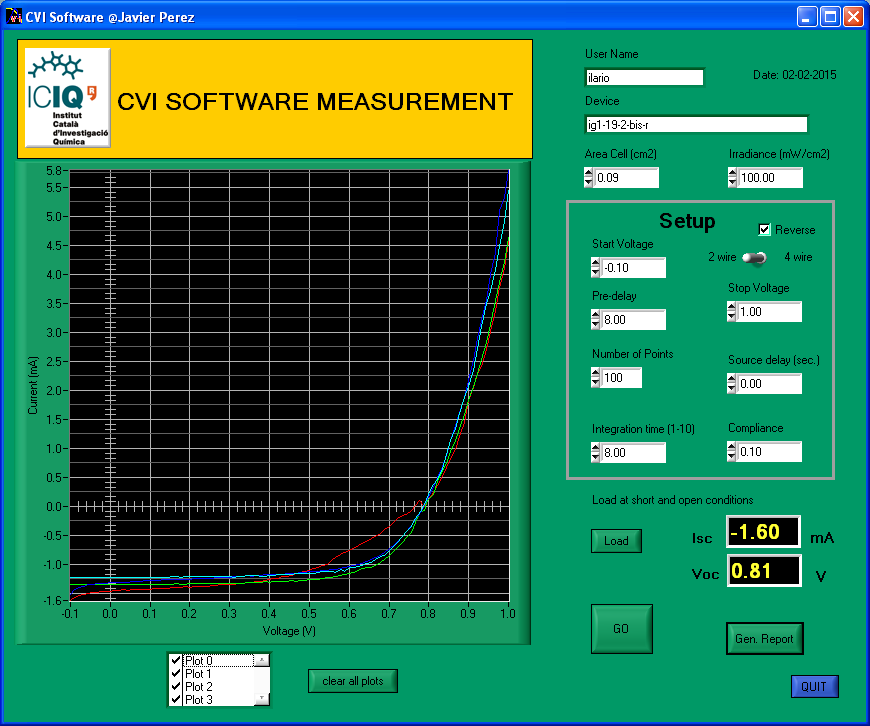
\includegraphics[width=0.7\textwidth]{old_iv_software/old_iv_software.png}
	\mycaption[Legacy software for current-voltage sweep measurement.]{}\label{fig:old_iv_software}
\end{SCfigure}

\paragraph{History of the project}
As a proof of concept, Dr.\ Daniel Fernandez Pinto developed in 2015 a Python library and a small \gls{gui} for communicating with Tektronix Keithley 2400 equipment \textsl{via} NI-VISA \cite{NationalInstruments2019} and running basic operations like current\hyp{}voltage sweeps.
I went on adding functions and expanding the \gls{gui} until obtaining a fully functional alternative to the legacy software shown in \cref{fig:old_iv_software}.
As far as I know, PyPV is currently used in the following research institutions: ICIQ (Institut Català d’Investigació Química), URV (Universitat Rovira i Vrigili), İzmir Katip Çelebi Üniversitesi, and Karamanoglu Mehmetbey University.

%I received a proof-of-concept software developed by  and decided to continue the development. At that point the software had an interface with few buttons and a working Keithley communication library.

\paragraph{User's requests}
The feedback from the new users of the software helped me improving PyPV in the following fields: solar simulator shutter control, more robust connection to the GPIB-USB-HS adapter, better installation instructions.

\subsection{Implementation and user interface}
\epigraph{\textit{"Ok, I finally completed it, by the way, why did you start developing this?"\\"Well, it was just a proof of concept, but it's nice you worked on it"}}

\paragraph{Autoscale} As it was explained in \cpageref{autoscale}, the automatic scale setting of the Keithley is detrimental for perovskite solar cells dynamic measurements.

\paragraph{Auto-measure}\label{automeasure}
The devices are kept under illumination at open circuit conditions, then a reverse sweep is measured and, immediately after this, the forward sweep is measured.
The reason for measuring the reverse sweep first, is that the reverse sweep starts from a high voltage point which is closer to the stabilized condition of the devices prior to the measurement (illuminated and open circuit).


\paragraph{Resistances} The shunt and series resistances estimation from current-voltage sweeps have been implemented but should not be considered for measurements on hysteretic devices, as explained in \cpageref{resistances}.

\paragraph{Scan speed calculation} 
The scan speed $s[V/s]$ is obtained from the voltage step \texttt{:SENSe:VOLTage:STEP} $V_|step|[V]$, integration time \texttt{:SENSe:VOLTage:NPLCycles} $n_|int|$ measured in power line cycles and the delay time \texttt{:SOURce:DELay} $t_|delay|[s]$ Keithley's parameters with the following \textit{empirical} expression:

\begin{equation}
s = \frac{V_|step|}{0.003 + t_|delay| + 0.06 \cdot n_|int|}
\end{equation}

where $t_|delay|$ is \SI{1}{\ms} for our measurement conditions \cite{Keithley2011}.

\subsection{Limitations}

The interface development has been started with the "Monkey Studio" software, which development has ceased even before the start of PyPV. This demonstrated to be a big failure in long term development planning.

\section{Robust and quick data analysis \textsl{via} R scripts}
\epigraph{\textit{"Is there an Origin version for Linux?"\\"No"}}

\subsection{Introduction}
To process the large amount of data which can be obtained using multiple techniques during the characterization of solar cells can be a very tedious and repetitive work.
I developed routines for data processing and representation, like fittings, integrations and plots.
I am describing the routines here in order to allow others to use and modify them.
All of the described functions can be downloaded from \url{https://github.com/ilario/photophysics-data-processing-R}.

\subsection{Helpers}
\paragraph{Set limits for axis and other parameters \texttt{limits_for_graphics.R}}
In this file I tried to centralize the parameters which should be edited by the user and will be used by the scripts.
This is for avoiding hardcoded values 

\paragraph{\texttt{devices-identification.R}}

\paragraph{\texttt{run-all-photophysics.R}}
\paragraph{\texttt{run-all-photophysics-comparisons.R}}
%\subsection{Photophysical Characterization \textsl{via} Optical and Electrical Transients}


\subsection{Charge Extraction (\glsentryshort{ce})}\label{r_ce}

\paragraph{\texttt{from_ce_to_table.R}}
\paragraph{\texttt{ce.R}}
\paragraph{\texttt{ce-subtractDark.R}}
\paragraph{\texttt{ce-integrateExp.R}}
\paragraph{\texttt{ce-from_output_to_graph.R}}
\paragraph{\texttt{ce-from_many_output_to_graph.R}}
\paragraph{\texttt{ce-time-many.R}}
\paragraph{\texttt{ce-with_limits.R}}

\subsection{Transient PhotoVoltage (\glsentryshort{tpv})}\label{r_tpv}

\paragraph{\texttt{from_tpv_tpc_to_table.R}}
\paragraph{\texttt{tpv-from_many_output_to_graph.R}}
\paragraph{\texttt{tpv-from_output_to_graph.R}}
\paragraph{\texttt{tpv-from_output_to_graph-with_limits.R}}
\paragraph{\texttt{tpv_onlyDeltaV.R}}
\paragraph{\texttt{tpv.R}}



\subsection{Transient PhotoCurrent (\glsentryshort{tpc})}\label{r_tpc}

\paragraph{\texttt{from_tpv_tpc_to_table.R}}
\paragraph{\texttt{tpc.R}}
\paragraph{\texttt{tpc-vs-tpv-vs-ce.R}}


\subsection{Differential Capacitance (\glsentryshort{dc})}\label{r_dc}

\paragraph{\texttt{dc-from_output_to_graph.R}}
\paragraph{\texttt{cedc.R}}
\paragraph{\texttt{dc-from_many_output_to_graph_capacitance.R}}
\paragraph{\texttt{dc-from_many_output_to_graph_charge.R}}

\subsection{Transient PhotoVoltage referred to charge from CE or DC (\glsentryshort{tpvce} and \glsentryshort{tpvdc})}\label{r_tpvcedc}


\paragraph{\texttt{tpvce-from_many_output_to_graph.R}}
\paragraph{\texttt{tpvce-from_output_to_graph.R}}
\paragraph{\texttt{tpvdc-from_many_output_to_graph.R}}


\subsection{Short circuit current reconstruction}

\cpageref{jsc_reconstruction}

\paragraph{\texttt{jrec-ce.R} and \texttt{jrec-dc.R}}

\subsection{Current-Voltage Sweeps}
\paragraph{\texttt{extractdata-curves-vi-separated_files.R}}
\paragraph{\texttt{iv-generate_mydata.R} and \texttt{iv-generate_mydata_with_comments.R}}
\paragraph{\texttt{iv-generate_images.R}}
\paragraph{\texttt{iv-generate_statistics.R}}
\paragraph{\texttt{iv-jsc_voc_vs_light_intensity.R}}
\paragraph{\texttt{iv-plot_list.R}, \texttt{iv-plot_list-suppinfo.R}, and \texttt{iv-light_intensity.R}}

\paragraph{\texttt{jsc-stability.R} and \texttt{voc-stability.R}}

\subsection{Other}
\paragraph{\texttt{mppt_to_graph.R}}
\paragraph{\texttt{profilometry.R}}
\paragraph{\texttt{tas-downsample.R}}
\paragraph{\texttt{tas-graph.R}}
\paragraph{\texttt{uvvis-pl.R}}

\section{Contributions to mppTracker}\label{software_mppt}
\epigraph{\textit{"A student of mine sells a complete system for that, just go and buy it"}}

As seen in \cpageref{characterization_hysteresis}, a \gls{mppt} system ensures to obtain a \gls{pce} value closer to the real world working conditions.
The hysteretic phenomena in perovskite solar cells requires new procedures for \gls{mppt} \cite{Cimaroli2017,Pellet2017} and a few commercial systems are already available for that \cite{CicciResearchsrl2019,CandlelightSystems}.
An interesting project for having robust \gls{mppt} measurable with Tektronix Keithley 2400 is mppTracker \cite{AFMD2017}.
I made a few contributions which are accessible on \url{https://github.com/AFMD/mppTracker/pulls?q=is%3Apr}.
	As the effort in this project were very limited on my side, I'll not further describe that.
	Recent reports on "bistable short circuit current" in perovskite solar cells by \authoryear{Calado2018} if confirmed would introduce local maxima making the \gls{mppt} system design even more complex.
